              
% ****** Start of file apssamp.tex ******
%
%   This file is part of the APS files in the REVTeX 4.1 distribution.
%   Version 4.1r of REVTeX, August 2010
%
%   Copyright (c) 2009, 2010 The American Physical Society.
%
%   See the REVTeX 4 README file for restrictions and more information.
%
% TeX'ing this file requires that you have AMS-LaTeX 2.0 installed
% as well as the rest of the prerequisites for REVTeX 4.1
%
% See the REVTeX 4 README file
% It also requires running BibTeX. The commands are as follows:
%
%  1)  latex apssamp.tex
%  2)  bibtex apssamp
%  3)  latex apssamp.tex
%  4)  latex apssamp.tex
%
\documentclass[%
 reprint,
%superscriptaddress,
%groupedaddress,
%unsortedaddress,
%runinaddress,
%frontmatterverbose, 
%preprint,
%showpacs,preprintnumbers,
%nofootinbib,
%nobibnotes,
%bibnotes,
 amsmath,amssymb,
 aps,
%pra,
%prb,
%rmp,
%prstab,
%prstper,
%floatfix,
]{revtex4-1}

\usepackage{graphicx}% Include figure files
\usepackage{dcolumn}% Align table columns on decimal point
\usepackage{bm}% bold math
\usepackage{hyperref}% add hypertext capabilities
%\usepackage[mathlines]{lineno}% Enable numbering of text and display math
%\linenumbers\relax % Commence numbering lines

%\usepackage[showframe,%Uncomment any one of the following lines to test 
%%scale=0.7, marginratio={1:1, 2:3}, ignoreall,% default settings
%%text={7in,10in},centering,
%%margin=1.5in,
%%total={6.5in,8.75in}, top=1.2in, left=0.9in, includefoot,
%%height=10in,a5paper,hmargin={3cm,0.8in},
%]{geometry}
\bibliographystyle{plain}

%\graphicspath{{C:\Users\Nick\Documents\GitHub\FYS2150\lab1}}

\begin{document}

%\preprint{APS/123-QED}

\title{FYS2150 \\
Lab Report: Time and Frequency}% Force line breaks with \\

\author{Nicholas Karlsen}
% \email{nichoka@student.matnat.uio.no}

\date{\today}% It is always \today, today,
             %  but any date may be explicitly specified



\begin{abstract}
  Studying the properties of linearly polarized light, and how one can determine the polarization of light by the use of polarization filters. Then studying how reflecting and transmitting light through a glass affects the polarization of light, and how this plays into the design of Polaroid sunglasses. Finally, studying the optical properties of crystalline calcite and how it can be used to rotate $\vec E$ in waveplates.
\end{abstract}

\maketitle
%\tableofcontents

\section{\label{sect:intro}Introduction}
  

\section{\label{sect:theory}Theory}
  
  \subsection{Polarization}

  \subsection{The Brewster angle}
    When light hits a reflective surface, it is partially reflected and transmitted. For a particular angle of incidence, light with which is polarized at paralell to the plane of incidence is fully transmitted. This angle is named the Brewster angle, $\phi_B$ and is defined mathemtaically in Eqn. \ref{eqn:brewster}. In particular, when a wave goes from Air to another medium, such as light, the equation simplifies to $\tan \phi_B \approx n_2$, as the refractive index of air is $n_{air}\approx 1$.
    \begin{equation}
        \tan \phi_B = \frac{n_2}{n_1}
        \label{eqn:brewster}
    \end{equation}

    

  \subsection{Birefringence}
    Certain materials, such as Calcite crystal exhibit birefringent behavior, where it effectively has two separate refractive indices for light polarized at right angle to each other, meaning that when unpolarized light is passed through the crystal, two displaced images will be visible. Birefringence can occur for different reasons, but in the case of crystalline Calcite, it is due to the uniaxial geometry of its lattice (See fig. \ref{fig:calcite}). Where light which is polarized is perpendicular to this optical axis will follow a certain, set refractive index, regardless of the crystals orientation. 

    \begin{figure}[h!]
      \center
      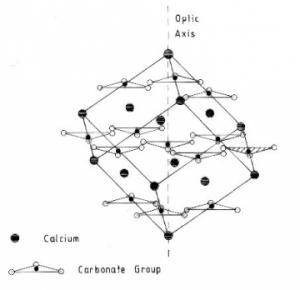
\includegraphics[width=8cm]{scripts/figs/calcite.jpg}
      \caption{Crystaline structure of calcite (\textbf{Source:} \url{http://lecturedemo.ph.unimelb.edu.au/Optics/Crystal-optics/Oh-1-Calcite-Crystal-Model/Calcite-Diagram})}
      \label{fig:calcite}
    \end{figure}

\section{\label{section:experimental}Experimental Procedure} 
  
  In order to minimize the effects that ambient light may have on the following experiments, the windows in the room were covered up and all lights not related to the experiment were turned off whilst data was being recorded, or observations were made.

  In all subsequent parts of this report, the spectral lamb to which i refer is a sodioum spectral lamp emitting close to monochromatic light of wavelength $\lambda=589$nm in air.

  \subsection{\label{subsect:polar_lamp}Checking the polarization of the spectral lamp}
    In order to determine whether or not the light emitted from the spectral lamp is polarized, the intensity of light was measured using a luxmeter\cite{data:luxmeter} after having gone through a polarization filter of variable angle acting as an analyzer, depicted in Fig \ref{fig:lux_ana_lamp}. When changing the angle of the analyzer, we defined a positive and negative direction, which was kept for all subsequent measurements using polarization filters. The angle of the polarization filter was changed in $10^\circ$ increments in the range $-90^\circ$ to $90^\circ$ and the intensity of the light measured by the luxmeter was noted for each angle.

    The uncertainty of the luminosity measured by the luxmeter in the range we measured is $\pm (5\% + 2\enspace \textup{digits})$ \cite{data:luxmeter}. However, in the presence of other ambient light sources the measurements taken in this, and subsequent measurements may not accurately reflect the intended nature of the experiment.


  \begin{figure}[h!]
    \center
    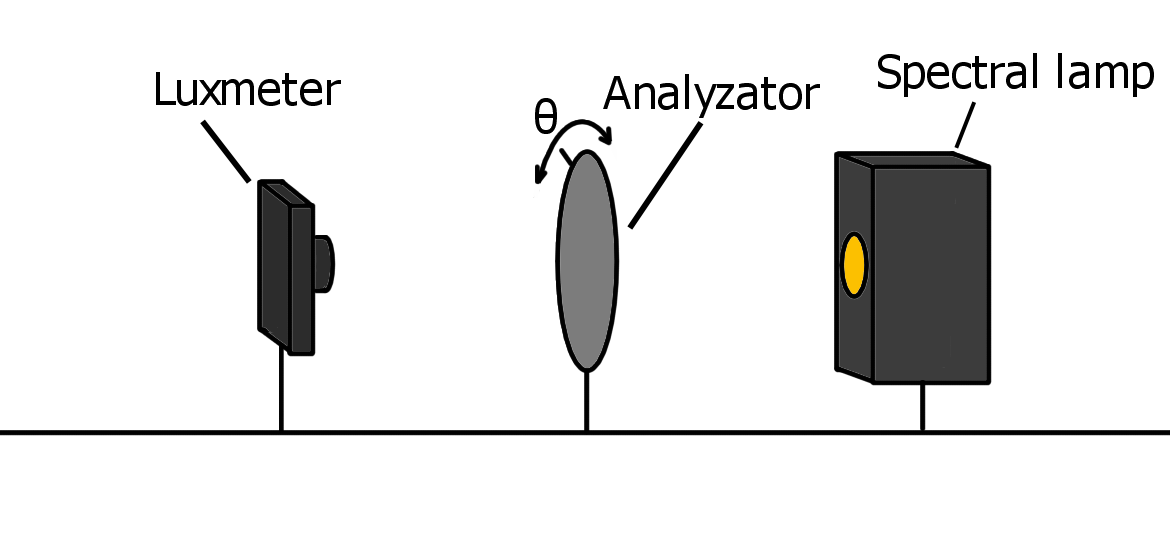
\includegraphics[width=8cm]{scripts/figs/diagram_1.png}
    \caption{Aparature to test the polarization of light emitted from a spectral lamp using a polarization filter with variable angle $\theta$ as an analyzer and measuring the intensity of the filtered light using the luxmeter. \textbf{Note:} Analyzer and Polarizer are misspelled in this and subsequent figures due to a poor translation of the terminology}
    \label{fig:lux_ana_lamp}
  \end{figure}

  \subsection{Testing Malus' law}

    In order to test Malus' law experimentally, we added a second polarization filter to our existing aperature (see sect. \ref{subsect:polar_lamp}), setting the first polarization filter to a fixed angle at $0^\circ$ whilst the second one is used as the analyzer, depicted in Fig. \ref{fig:lux_ana_pola_lamp}. In order to minimize the effects that ambient light and other potential contaminants, the apparatus was kept as tightly stacked as possible. The intensity registered by the luxmeter was again measured in $10^\circ$ increments in the range $-90^\circ$ to $90^\circ$ which was noted in the lab journal. 

    \begin{figure}[h!]
      \center
      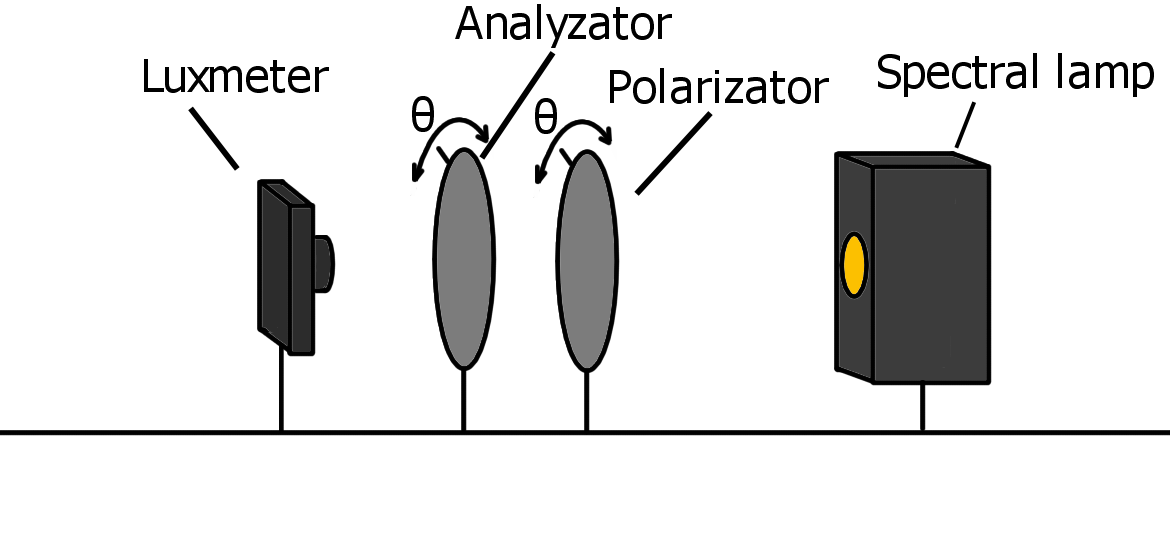
\includegraphics[width=8cm]{scripts/figs/diagram_2.png}
      \caption{Aparature to test Malus' law, where the polarizer is kept at a constant angle while the analyzer is varied.}
      \label{fig:lux_ana_pola_lamp}
    \end{figure}

    Afterwards, a third polarization filter was placed after the analyzer and set to a fixed angle at $90^\circ$ (see Fig. \ref{fig:lux_pola_ana_pola_lamp}). The angle of the analyzer was once again varied as before, and the intensity recorded by the luxmeter was noted in the journal.

    \begin{figure}[h!]
      \center
      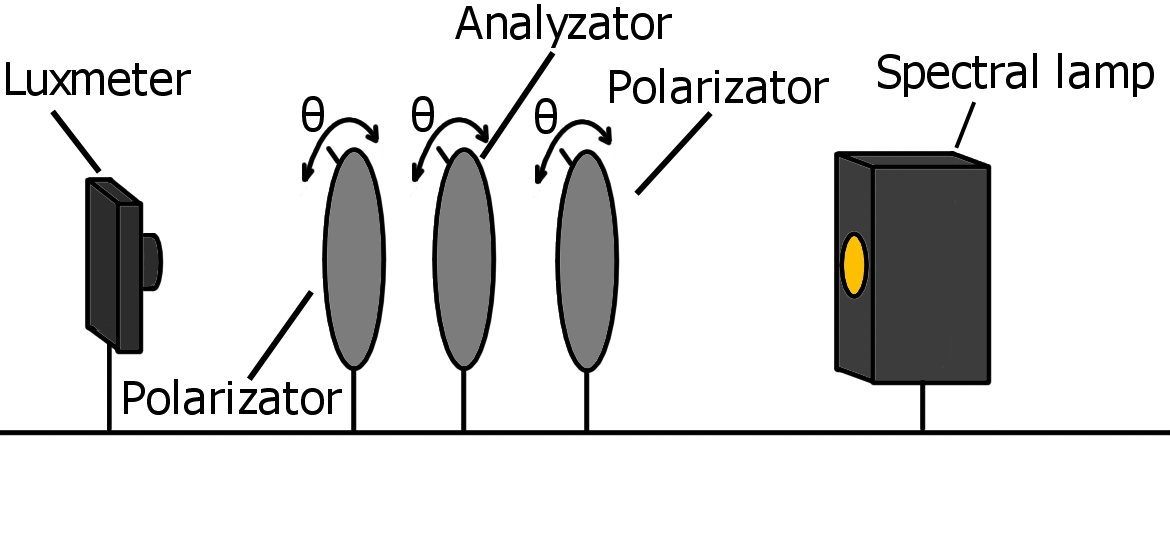
\includegraphics[width=8cm]{scripts/figs/diagram_3.png}
      \caption{Alternative aparature to test Malus' law, where the two polarizers are kept at a constant angle while the analyzer is varied.}
      \label{fig:lux_pola_ana_pola_lamp}
    \end{figure}

    \subsection{Reflection of polarized light\label{subsect:reflection_experimental}}
      In order to test how the intensity of S and P-polarized light, reflected from a prism with a varying angle of incidence, a modified spectroscope was used as shown in Fig. \ref{fig:mod_spectro}. the angle, and intensity was recorded digitally on a computer using capstone. The angle recorder only measured the change in angle from starting the recording, so there was a notable uncertainty in zeroing the apparatus before starting. The sights, used to read the angle manually were blocked by a cable, such that it could not be used properly, and the geometry of the spectrometer itself was not perfect. For large angles, i.e when the incident line is nearly parallel with the plane of reflection, it was observed that some of the light was transmitted through the prism rather than being reflected. This is likely due to the prism not being properly aligned with the laser, which was reflected in the results. As such, the data for large angles $\phi$ do not follow what is expected, which must be taken into account when reading the results.

      As for making the measurements, the polarisator was set either parallel or tangential to the reflective plane of the prism and the prism was adjusted such that the reflective plane was paralell to the laser beam. Captstone was then started and the luxmeter and prism were slowly rotated untill the angle between the laser and the luxmeter was roughly $65^\circ$. This was repeated for both S and P-polarized light.

      Afterwards, we investigated the direction of transmission of a pair of polaroid glasses using an analyzer. The analyzer was rotated and the change in intensity of light was observed through the polaroid glasses.

    \begin{figure}[h!]
      \center
      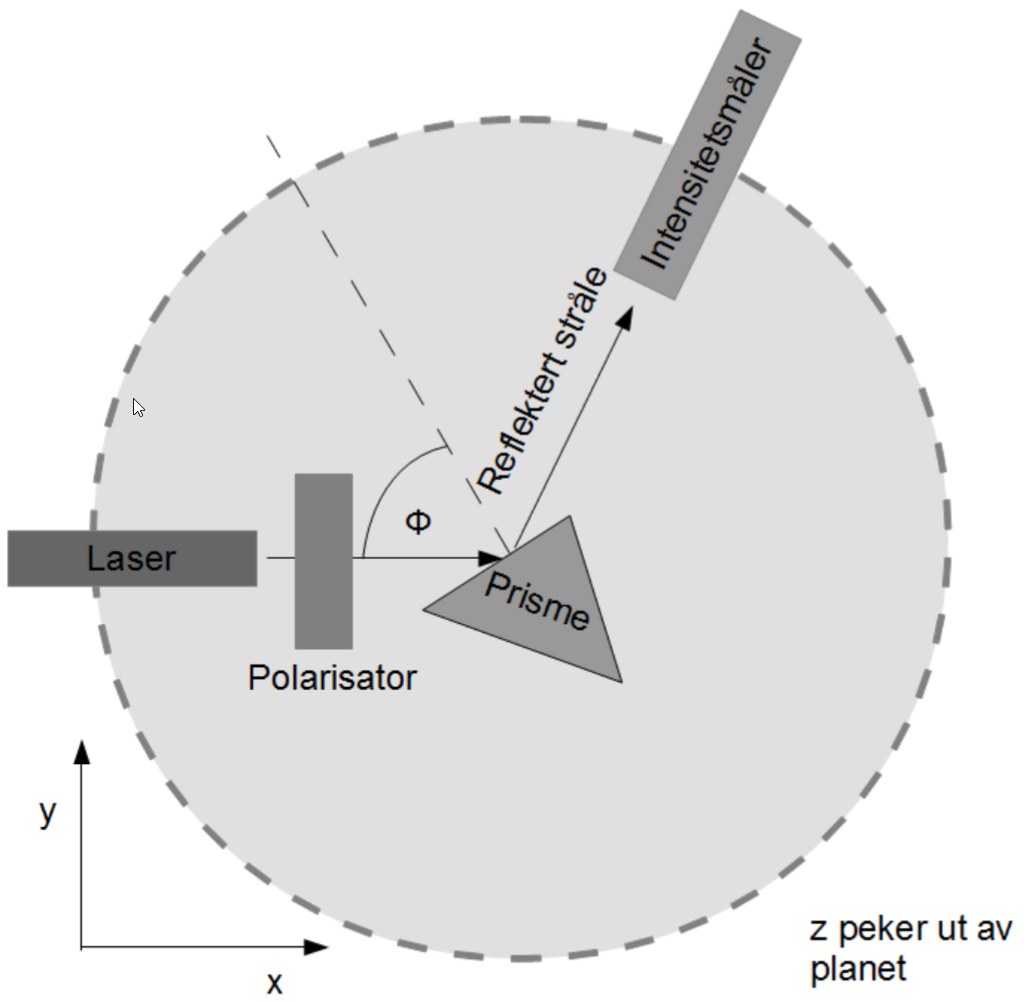
\includegraphics[width=8cm]{scripts/figs/modified_spectrometer.png}
      \caption{Modified spectrometer used to test how the intensity of reflected, polarized light changes with the angle of incidence.}
      \label{fig:mod_spectro}
    \end{figure}

  \subsection{Light transmitted through an angled glass plate}

    In order to investigate how light is transmitted through a glass plate, we used an aparature as the one depcited in Fig. \ref{fig:glassplate}. The glass plate was oriented tangentilly to the incoming, unpolarized light beam, and the angle which it made in the direction paralell to the beam could be adjusted. There was also a anglemeasurer with a maker which allowed us to read the angle which the glass plate had to the vertical axis. It was also noted that the glass plate used is of the same material as the prism used in section \ref{subsect:reflection_experimental}.

    The distance between the single slit and convex lens was adjusted untill the line projected onto the screen was in focus.

    Afterwards, the polarization of the light after having passed through the glass plate was then observed by adjusting the analyzer for different angles of the glass plate. In particular, we adjusted the glass plate to the brewster angle which was found for the prism in section \ref{subsect:reflection_experimental}.

    \begin{figure}[h!]
      \center
      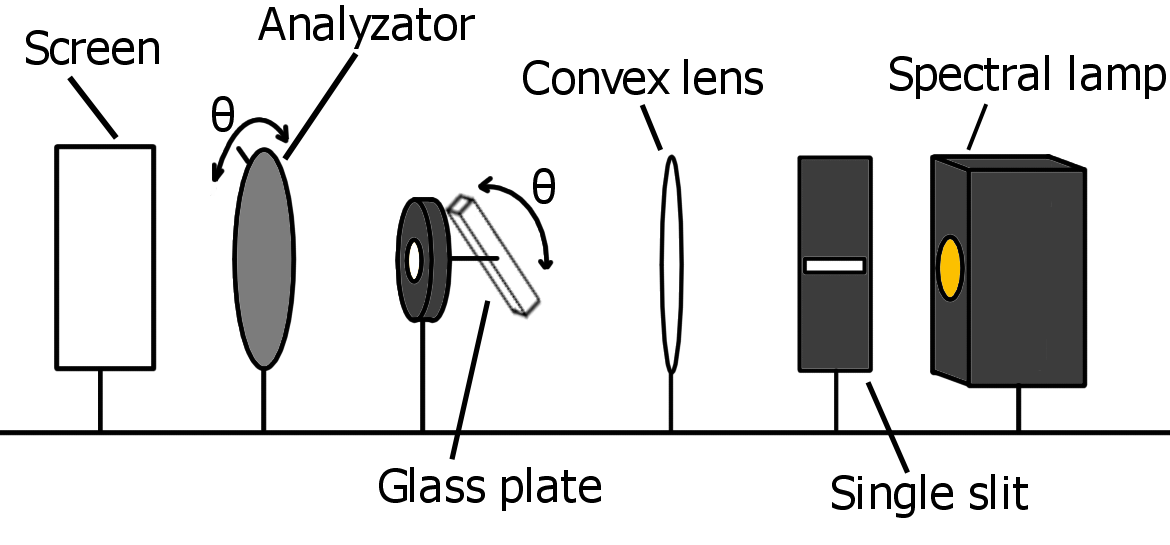
\includegraphics[width=8cm]{scripts/figs/diagram_4.png}
      \caption{}
      \label{fig:glassplate}
    \end{figure}

  \subsection{Observing birefringence in crystalline Calcite}
    We had two samples of crystalline calcite. One of which was naturally occurring sample, and another which was cut tangentially to its optical axis on two opposing sides. Both of the crystals were transparent, and text was clearly readable when looking through them. The crystals were placed on an illuminated panel, on top of which was some text printed on transparent plastic. We then observed the text by looking through the two calcite crystals, both with and without a polarization filter acting as an Analyzer. 

    Afterwards, we used an aparature as the one depicted in Fig. \ref{fig:calcite} to investigate how the crystals affected a thin beam of light which is passed through it. The crystals were held inbetween the analysator and lens, and we investigated how the intensity of the dots projected on the screen varied as we changed the angle of the analyzer.

    \begin{figure}[h!]
      \center
      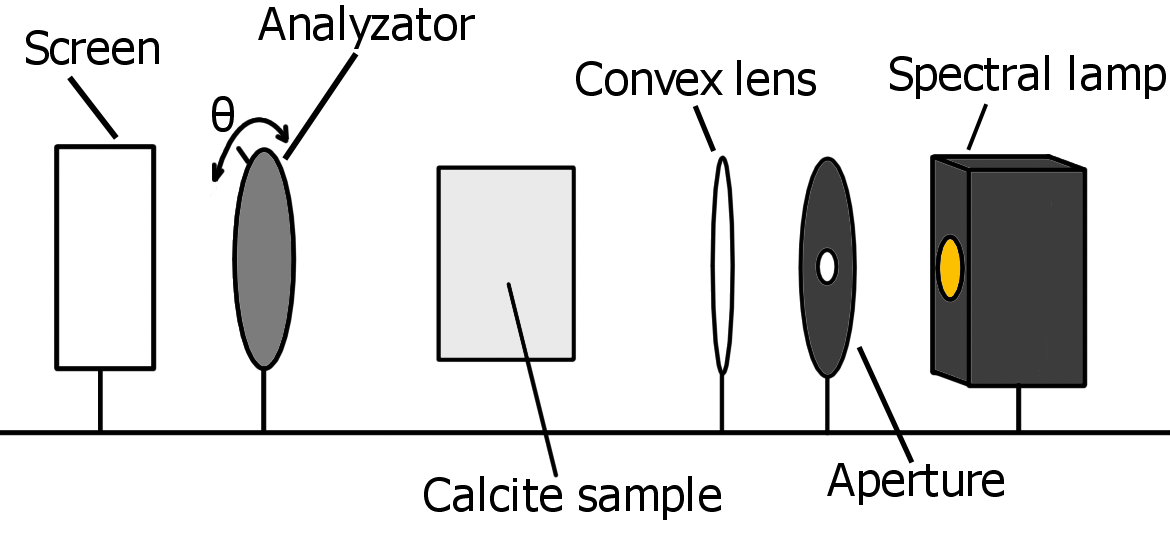
\includegraphics[width=8cm]{scripts/figs/diagram_5.png}
      \caption{Aperature used to test both the qualitative effects on a thin beam of light being passed through a calcite sample as well as the polarization of this light, which is projected onto the screen.}
      \label{fig:calcite}
    \end{figure}

  \subsection{Circular polarization of light using Calcite waveplates}
    In order to investigate the effect of the polarization of light emitted by the spectral lamp when passed through $\lambda /2$ waveplates, where $\lambda=550$, the most abundent wavelength of visible light emitted from the sodium spectral lamp, an aparature as depicted in Fig. \ref{fig:waveplate} was prepared. The aparature allowed for the rotation of the waveplates along the axis paralell to the light being passed through it from the spectral lamp. There was however no markings on the waveplate to indicate its current orientation, which had to be determined by a methodic approach by the use of the analyzer.

    \begin{figure}[h!]
      \center
      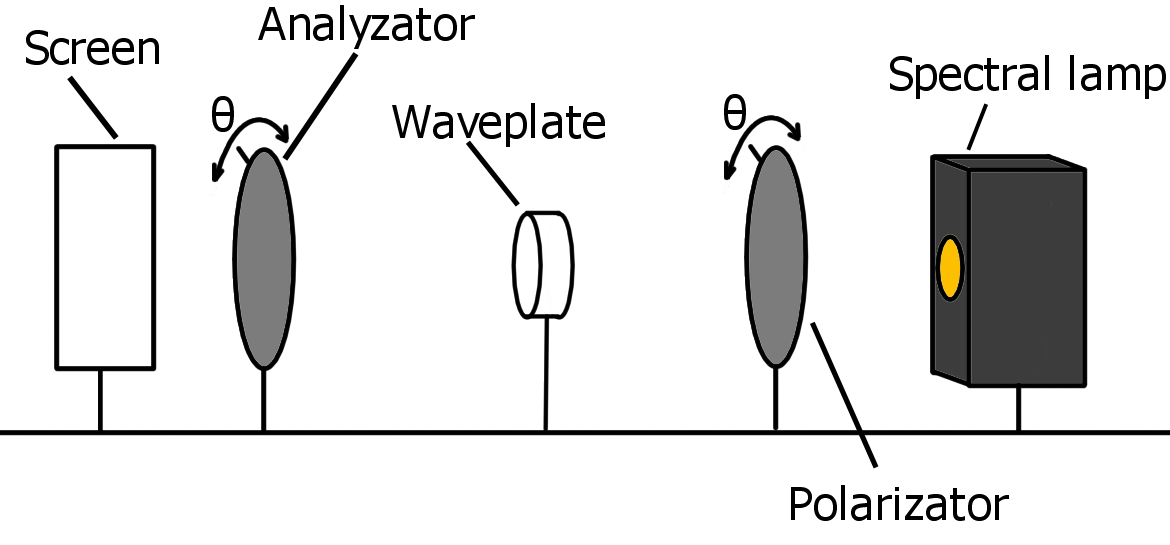
\includegraphics[width=8cm]{scripts/figs/diagram_6.png}
      \caption{Aparature used to investigate how a calcite waveplate affects the polarization of polarized light}
      \label{fig:waveplate}
    \end{figure}

    The polarizer was set to $0^\circ$ and the analyzer to $+90^\circ$. The waveplate is then rotated untill the projected image was at a minima. As we did not have a luxmeter, this was purely based on the observed intensity of the projection on the screen. When the intensity minima is reached with this configuration, the optical axis is at either $0^\circ$ or $90^\circ$ to the vertical axis. We then adjusted the polarizer to $+45^\circ$ and observed how the intensity of the projected light varied when adjusting the analyzer to different angles.

    Afterwards, we added a second $\lambda/4$ waveplate to the aparature, which in combination effectively yields a $\lambda/2$ waveplate. The polarizer was then set to $+45^\circ$ and the analyzer to $-45^\circ$. We then turned the newly added waveplate, while leaving the old one in its previous orientation. The new waveplate was turned untill the projected light reached an intensity maxima. Again, the when this maxima occured was based on our judgement, as no quantitative measurement regarding its intensity was made. When the maxima was reached, the analyzer was turned to $+45^\circ$ and the intensity of the projected light was at a minimum.
    


\section{\label{sect:results}Results}
  
  \subsection{Polarization of light emitted by the spectral lamp}

  The polarization of light emitted by the Sodium spectral lamb was investigated using an analyzer, and measured intensities using the luxmeter is presented in Table \ref{tab:ana}. A graph of this data is also provided in Fig. \ref{fig:ana_plot} for added clarity.

  \begin{table}[h!]
      \center
      \caption{Measured intensity when passing unpolarized light through a single polarization filter, $\theta$ denoting the angle of the filter. Aparature depicted in Fig. \ref{fig:lux_ana_lamp}. A graph of this data set is shown in Fig. \ref{fig:ana_plot}}
       \begin{tabular}{r | l}
        $\theta$ [deg] & Intensity [Lux] \\ \hline
         \input{scripts/data/ana.dat}
       \end{tabular}
       \label{tab:ana}
  \end{table}

  \begin{figure}[h!]
    \center
    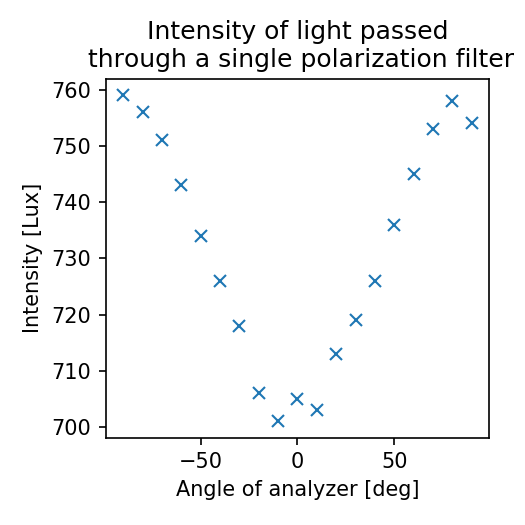
\includegraphics[width=8cm]{scripts/polartest.png}
    \caption{Graphical depiction of the data presented in table \ref{tab:ana}}
    \label{fig:ana_plot}
  \end{figure}

  \subsection{Confirming Malus law}

  The measured intensities measured of $0^\circ$ polarized light for different angles $\theta$ of an analyzer, as depicted in Fig. \ref{fig:lux_ana_pola_lamp} is presented in Table \ref{fig:malus1} such that it should satisfy the proportionality $I \propto \cos^2(\theta)$ in accordance with Malus law. In addition to the measured data points, there is also a linear fit with its errors $\delta m, \delta c$.


  \begin{figure}[h!]
    \center
    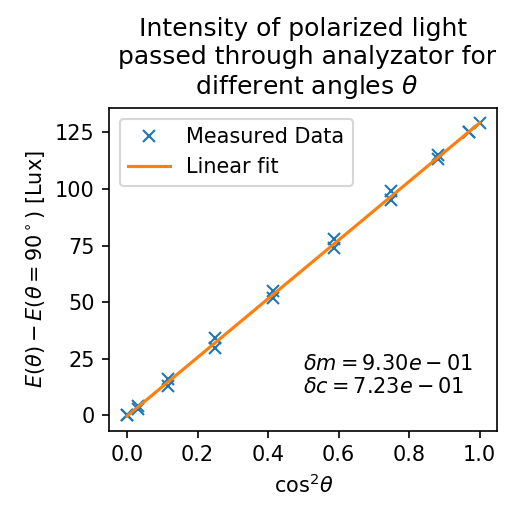
\includegraphics[width=8cm]{scripts/malus1.png}
    \caption{$E(\theta)$ denotes the intensity of light measured by the luxmeter as a function of the angle of the analyzer. $\delta m$ and $\delta c$ denote the error of the constants $m$, $c$ in the linear fit of the form $y=mx+c$.}
    \label{fig:malus1}
  \end{figure}

  Following, in Fig. \ref{fig:malus2} are the intensity measurements presented as a function of the angle of the analyzer in the aparature depicted in \ref{fig:lux_pola_ana_pola_lamp} where light is first polarized at $0^\circ$, passed through an analyzer of variable angle $\theta$, polarized again at $+90^\circ$ before its intensity is measured by the luxmeter.
  
  \begin{figure}[h!]
    \center
    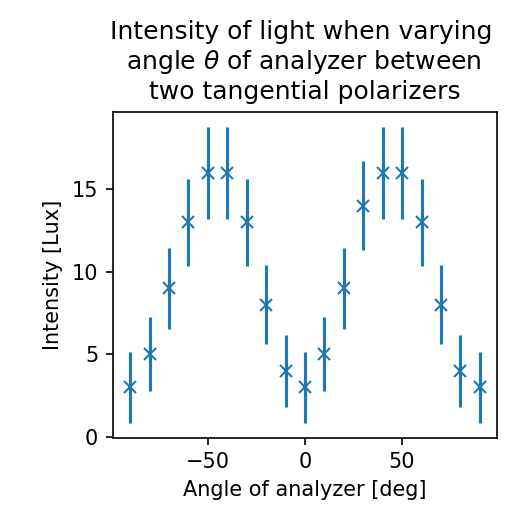
\includegraphics[width=8cm]{scripts/malus2.png}
    \caption{Intensity of light measured by luxmeter for different angles $\theta$ of analyzer which is positioned between two tangential polarizers at angles $-90^\circ$, $0$ respectively. See Fig. \ref{fig:lux_pola_ana_pola_lamp}}
    \label{fig:malus2}
  \end{figure}


  \subsection{Intensity of reflected light for S and P polarized light \label{sect:res_prism}}

  The intensities for P and S polarized light reflected off a prism at different angles $\theta$ are presented in Figures \ref{fig:ppolar}, \ref{fig:spolar} respectively. In both graphs, the angle on the $x$-axis does not match the angle $\phi$ in Fig. \ref{fig:mod_spectro}, but rather $\phi + 90^\circ$. Additionally, the data prior to the primary peak in all plots have been left in, but should be ignored for reasons explained in section \ref{subsect:reflection_experimental}, as they deviate from the theoretical model due to flaws in the apparatus.

  \begin{figure}[h!]
    \center
    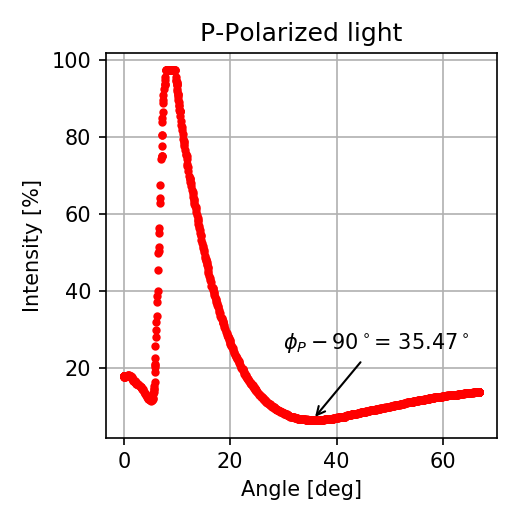
\includegraphics[width=8cm]{scripts/ppolar.png}
    \caption{Intensity profile due to p-polarized light, where $\phi_P$ denotes the Brewster angle. Note that the measurements for angles prior to the peak are to be ignored as discussed in the experimental section.}
    \label{fig:ppolar}
  \end{figure}

  \begin{figure}[h!]
    \center
    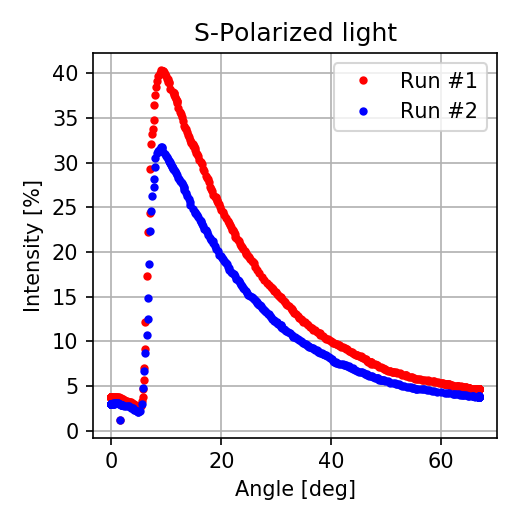
\includegraphics[width=8cm]{scripts/spolar.png}
    \caption{Intensity profile due to p-polarized light from two separate attempts of the experiment. Note that the measurements for angles prior to the peaks are to be ignored as discussed in the experimental section.}
    \label{fig:spolar}
  \end{figure}

  \subsection{Polarization of light transmitted through glass plate}
    Using an apparatus as depicted in Fig. \ref{fig:glassplate}, we observed the polarization of light transmitted through the glass plate at different angles of incidence. When the glass plate was vertical such that the angle of incidence was $0^\circ$, there was no change in the intensity of the projected light when changing the angle of the analyzer. 

    The angle of incidence was then adjusted to the equivalent of the Brewster angle for the glass prism (see sect. \ref{sect:res_prism}), roughly $34^\circ$. For this angle, we observed an intensity maxima when the analyzer was at $0^\circ$ and a decreasing intensity as we slowly adjusted the analyzer in the positive and negative directions, reaching an intensity minima at both $\pm 90^\circ$. 

  \subsection{Observations when looking at light passed through crystalline Calcite}
    When observing text through the naturally occurring sample of crystalline calcite, the birefringence of calcite was observed by the text splitting into two, seemingly identical copies of each other. When placing a the small polarization filter on top of the crystal and turning it, there were specific angles in which the text disappeared, one for each image. Without making any measurements, these angles seemed to be roughly $90^\circ$ relative to each other. Meaning the two images of the text are tangentially polarized relative to each other. 

    When placing the sample in the apparatus depicted in Fig. \ref{fig:calcite}, there were two small circles of light projected onto the screen when the analyzer was set to $0^\circ$ and $90^\circ$.  Setting the analyzer to $+45^\circ$ resulted in one of the circle disappearing, and setting it to $-45^\circ$ made the other circle disappear.

    When looking at the fabricated calcite sample, which was cut tangential to its optical axis. Only one image of the text was visible, and rotating a polarizing filter on top of it had no visible effect on the image. When investigating further, again using the apparatus depicted in Fig. \ref{fig:calcite}, there was only one circle projected onto the screen and rotating the analyzer had no visible effect on its luminosity. 

  \subsection{Observations on the intensity of light polarized with calcite waveplates}
    When the $\lambda/4$ waveplate was oriented such that its optical axis was at either $0^\circ$ or $90^\circ$ to the vertical axis in the apparatus depicted in Fig. \ref{fig:waveplate}, the polarizer was then set to $+45^\circ$. Then, any adjustments made to the analyzer had no visible impact on the luminosity of the light projected onto the screen.

    Following, a second $\lambda/4$ waveplate was added next to the previous, effectively yielding a $\lambda/2$ waveplate. The polarizer was then set to $+45^\circ$ and the analyzer to $-45^\circ$. The newly added waveplate was then rotated until there luminosity of the projected light reached a maxima. The analyzer was subsequently set to $+45^\circ$, which resulted the luminosity of the projected light reaching a minima. implying that the direction of the $\vec E$ field had been rotated by $90^\circ$ after having traversed the waveplates.

\section{\label{sect:discuss}Discussion}
  \subsection{Polarization of spectral lamp}
    Whilst suggested it was suggested that the light emitted from the sodium spectral lamp emitted unpolarized, mostly monochromatic light, the data in Fig. \ref{fig:ana_plot} seems to suggest otherwise, that a small component, roughly 10\%, of the light is polarized in the horizontal axis. However, this data could also be explained by some ambient light source containing polarized light. In retrospect, recording the background luminosity when the spectral lamp turned off would have been a good idea, as it would provide an easy answer to this question.

    However, the data in Fig. \ref{fig:malus2} also hints at the presence of a systematic error. When filtered through two tangential polarizers, one expects zero intensity. A third possibility, is also that the polarization filters simply aren't perfect and allows some light of different polarization pass through. It was noted in the lab journal that there were "small bright holes" in the filters, which does strengthen my suspicion that this is the cause of this unexpected behavior.

  \subsection{Relative intensities of S and P polarized light in reflections}
    As shown in the data presented in figures \ref{fig:ppolar}, \ref{fig:spolar}. When light is reflected off a glass surface, the component of light which is polarized parallel with the plane of incidence has in general, a larger relative intensity compared to tangentially polarized light. This comes into play in the manufacture of Polaroid sunglasses, which as seen are polarized in the vertical axis, which in most circumstances is parallel to the plane of incidence of light reflected from such things as puddles of water, or the ocean. The latter of which of particular interest to anyone who might travel at sea, where a large amount of sunlight will be reflected from the surface of water, the largest relative amount of which is P-polarized light.

    This was again observed when investigating the transmittance of polarized light through a glass plate for different angles of incidence. When the angle of incidence was 0, the transmittance was seemingly not affected by the polarization of light. However, when changing the angle to correlate to the Brewster angle of the material, it was observed that the intensity of the projected P-polarized light was was at a maximum, implying that the majority of the P-polarized light was transmitted through the plate rather than being reflected. However, the S-polarized light was nearly invisible, meaning most of it was reflected of the prism. In this particular scenario, the Polaroid glasses would be rather ineffective, as a large portion of the P-polarized light would be transmitted, filtering out the S-polarized light would be more desirable. This could of course easily be accomplished by simply tilting ones head by $90^\circ$.


\section{\label{sect:conclusion}Conclusion}
  The experiments 

\newpage
\bibliography{references_rep6.bib}

%%%%%%%%%%%%%%%%%%%%%%%%
%%% END OF MAIN BODY %%%
%%%%%%%%%%%%%%%%%%%%%%%%
\end{document}
%
% ****** End of file apssamp.tex ******
              